\documentclass[a4paper, 11pt]{article}
\usepackage{comment} % enables the use of multi-line comments (\ifx \fi) 
\usepackage{fullpage} % changes the margin
\usepackage[margin=35pt]{geometry}
\usepackage{graphicx}
\usepackage{microtype} 
\usepackage{titlesec}
\usepackage{color, colortbl}
\usepackage[table]{xcolor} 
\usepackage[numbers,super]{natbib}
\usepackage{bibentry}
\nobibliography*

%\usepackage[most]{tcolorbox}

%\usepackage{fontspec}
%\setmainfont{Georgia} 
\titleformat*{\section}{\large\bfseries}

\begin{document}

\noindent
\large\textbf{Committee Meeting Report} \hfill \textbf{Sahar Mozaffari} \\
\normalsize  \hfill Professor: Carole Ober  \\
GGSB Matriculated 2013 \hfill Date: 10/02/17 \\
\noindent\makebox[\linewidth]{\rule{\paperwidth}{0.4pt}}

\large\textbf{\\Progress since last Committee Meeting - September 8, 2016}
\subsection*{Awards}
% Horizontal line after name; adjust line thickness by changing the '1pt'
\begin{itemize}
    \item ASHG Reviewer's Choice Abstract Award  \hfill 2016 \& 2017
    \item Awarded \& Renewed F31 Ruth L. Kirschstein NRSA \hfill 9/2016-9/2018
    \item FASEB MARC Travel Award to ASHG \hfill 2014 \& 2015 
    \item Genetics and Regulation Training Grant \hfill 2013-2016
\end{itemize} 

\subsection*{Publications}
\begin{itemize}
    \item Submitted to PeerJ: \bibentry{Hart:2017vg}
    \item Revising: \bibentry{Mozaffari:dg}
    \item Under revision Scientific Reports: \bibentry{Igartua:2017fg}
    \item \bibentry{Gamazon:2015fa}
\end{itemize}

\subsection*{Oral Presentations}
\begin{itemize}
	\item GGSB Work in Progress \hfill April 2016 \& March 2017\\ \emph{Parent of Origin Effects in the Hutterites}
%	\item Genetics of Model Organisms Club \hfill April 21, 2016\\  \emph{Parent of Origin Effects in the Hutterites}
  	\item Human Genetics Work in Progress \hfill January 20, 2016\\ \emph{Parent of Origin Effects} 
	\item Molecular Biosciences Retreat \hfill November 5, 2015\\ Mozaffari SV, DeCara J, Shah S, Herman C, Lang R, Nicolae D, Ober C., \emph{Parent of Origin GWAS with Cardiovascular Disease Associated Traits in the Hutterites.} 2015: Nov 5; Galena, IL.
    \item ASHG\hfill October 9, 2015\\ Mozaffari SV, DeCara J, Shah S, Herman C, Lang R, Nicolae D, Ober C., \emph{Parent of Origin GWAS of CVD-Associated Phenotypes in the Hutterites} (Abstract Program \#310). Presented at the Annual Meeting of The American Society of Human Genetics; 2015: Oct 9; Baltimore, MD. 
  

\end{itemize}

\subsection*{Posters}
\begin{itemize}
    \item Mozaffari SV, Nicolae D, Ober C. \emph{Opposite Allele Parent of Origin Effects on Cardiovascular and Asthma Associated Traits in the Hutterites}. Poster presented at the Gordon Research Seminar and Conference; 2017: July 8-14; Stowe, VT
    \item Reviewer's Choice Abstract Award: \\Mozaffari SV, Nicolae D, Ober C. Opposite Allele Parent of Origin Effects on Body Mass Index in the Hutterites. Poster presented at the Annual Meeting of The American Society of Human Genetics Conference; 2016: Oct 18-22; Vancouver, Canada
    \item Mozaffari SV, Gamazon E, Aquino-Michaels K, Cox NJ, Im HK. \emph{Quantifying Context Specificity of Gene Regulation using Predicted Gene Expression Levels.} Poster presented at the Annual Meeting of The American Society of Human Genetics Conference; 2014: Oct 18-22; San Diego, CA 

\end{itemize}

\subsection*{Teaching Assistantship Requirements Completed}
\begin{itemize}
	\item HGEN 47000 \emph{Human Genetics} \hfill Fall 2015 \& 2017\\
- Graduate Course: Classic and modern approaches to studying cytogenetic, Mendelian, and complex human diseases. Grant proposal writing course. \\ - Fall 2017: Conducting two-day computational workshop on GWAS
    \item MGCB 31400 (BIOS 21236) \emph{Genetic Analysis of Model Organisms}\hfill Fall 2014\\
- Graduate \& Undergraduate Course: Introduction to genetic tools, experiments, and model organisms 
\end{itemize}



\subsection*{Additional Courses}
\begin{itemize}
    \item STAT 24500 \emph{Statistical Theory \& Methods II }\hfill Winter 2015
    \item HGEN 46900 \emph{Human Variation \& Disease} \hfill Spring 2015
    \item STAT 35500 \emph{Statistical Genetics} \hfill Spring 2015
    \item myChoice Mini-Course: \emph{Effective Writing in the Biological Sciences} \hfill Fall 2015
    \item HGEN 48600 \emph{Fundamentals of Computational Biology: Models \& Inference} \hfill Winter 2016
    \item PBHS 31831 \emph{Genetic \& Molecular Epidemiology} \hfill Spring 2016
  
	
\end{itemize}

\subsection*{Additional Workshops \& Conferences}
\begin{itemize}
	\item ComSciCon Chicago (Communicating Science Conference \& Workshop)  \hfill August 2017
	\item Gordon Research Seminar \& Conference: Human Genetics \& Genomics \hfill July 2017 \\ Discussion Leader for mentorship session at GRS
     \item Summer Institute in Statistical Genetics at the University of Washington \hfill July 2016
        \item Master R Developer Workshop taught by Hadley Wickham \hfill May 2015
\end{itemize}

\subsection*{Extracurricular}
\begin{itemize}
	\item myCHOICE Data Science Trek to San Francisco Bay Area \hfill November 2017
	\item Museum of Science \& Industry: Science Connections volunteer \hfill Fall 2014-current \\
		Introduce genetic concepts to guests in a fun and engaging way, incorporating hands-on activities.\\Assist in the Fabrication Lab helping guests design and print custom objects using 3D printers and laser cutters.
	\item UChicago Software Carpentry Helper \hfill Fall 2015, 2016, \& 2017
	\item Expanding Your Horizons (EYH) Chicago: volunteer \hfill March 2017 \\
	Engage, inspire, and empower young girls to pursue STEM careers at a one-day STEM symposium where 300 middle school girls participate in hands-on science, technology, engineering and math led by academic and professional women.
   	\item myCHOICE Internship: Institute of Translational Medicine: writer \hfill Summer 2015\\Translate complex research into dynamic science stories. Share translational research stories in weekly newsletter, ITM website, and social media platforms

\end{itemize}



%\noindent\makebox[\linewidth]{\rule{\paperwidth}{0.4pt}}

%\section*{Attachments}
%Make sure to change these
%Lab Notes, HelloWorld.ic, FooBar.ic
%\fi %comment me out
\newpage

%\noindent\makebox[\linewidth]{\rule{\paperwidth}{0.4pt}}
\section*{Proposal Updates:} %\begin{tcolorbox}[colback=white,colframe=red!75!black]
\textbf{AIM 1a} To identify and characterize parent of origin effects on quantitative traits in the Hutterites. 
\textbf{\\AIM 1b} To estimate maternal and paternal heritability measures on quantitative traits in the Hutterites.\\
 \textbf{\\AIM 2a} To identify and characterize parent of origin effects on gene expression in 430 Hutterites.\\
\textbf{AIM 2b} To identify and characterize parent of origin and allele specific effects on gene expression in 430 Hutterites.\\
\textbf{\\Since my last Committee Meetng}
\textbf{\\AIM 1a}\\
	Completed with preprint on bioRxiv \cite{Mozaffari:dg}, working on revising and resubmitting. We are trying to replicate the significant opposite effects of SNPs in birth weight in the Hutterites.
\textbf{\\AIM 1b}\\
  	Currently working on, adapting methods published in Mott \emph{et al.} \cite{Mott2014}. Last committee meeting, it was established this would be the last aim I work on .
%\begin{figure}[!h]
%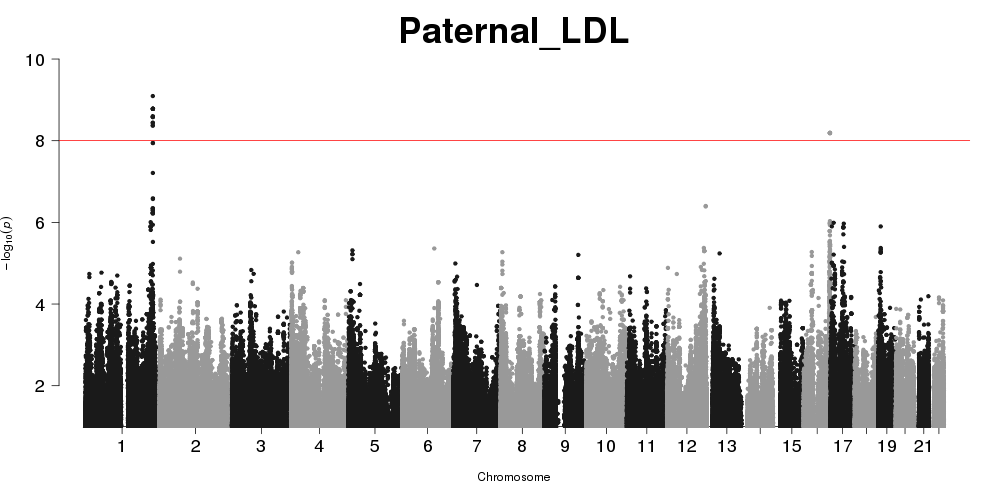
\includegraphics[width=0.5\textwidth]{Manhattan_paternal_LDL_8_17_16.png}
%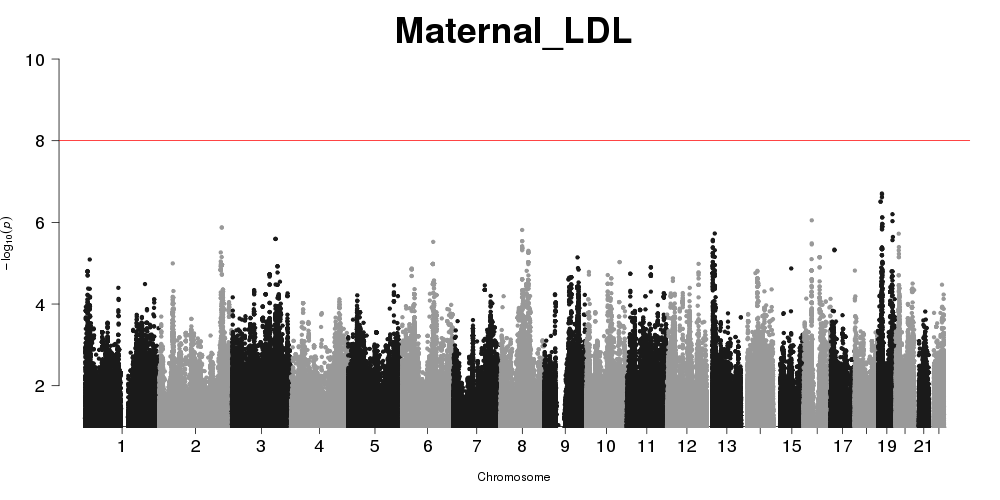
\includegraphics[width=0.5\textwidth]{Manhattan_maternal_LDL_8_17_16.png}
%\caption{\label{fig:POGWAS}Paternal and Maternal allele PO- GWAS Manhattan plots for LDL.}
%\end{figure}

\textbf{\\AIM 2a}\\
I have remapped the LCL RNA-seq data (and whole blood data for replication) using STAR\cite{Dobin:2012fg} and corrected sample swaps using verifyBamID.\cite{Jun:2012je} I used WASP\cite{vandeGeijn:2015hi} to remove mapping bias and remove duplicate reads. I then mapped reads to the maternal ($Y_m$) and paternal ($Y_p$) haplotypes. I used STAR to measure gene count from reads. I removed lowly expressed genes but did not normalize gene expression or remove covariates since comparing maternal and paternal expression is done in the same sample under the same conditions. \\
\\For this aim I am using simple binomial tests to detect patterns of parent of origin effects (i.e. imprinting) using maternal and paternal gene expression but not any SNPs (no POeQTL). (Removed duplicate reads so no need to model overdispersion). 
First, I can test for directional asymmetry to test if any genes have maternal or paternal effects by generating a binomial Z-score for each subject for each gene. I only use individuals where $Y_p+Y_m=5 $ and $Z_i \neq 0 $ to get a statistic of how skewed the gene expression is for each gene using a binomial test. 
\begin{equation}\label{Zscore}
	Z_i= \frac{(Y_p^{i}-Y_m^{i})}{\sqrt(Y_p^{i}+Y_m^{i})}
\end{equation}
\begin{equation}\label{signtest}
	S \sim Bin(\# subjects, \frac{1}{2}) 
\end{equation}

Second, I test for asymmetry in maternal and paternal gene expression by genes and weighing by library size where $w_i \propto \frac{1}{library size_i} $ and $ w_i = \frac{10millionreads}{\#ofreads_i} $\\
\begin{equation}\label{my_first_eqn}
	Z_g= \frac{\sum_{i=1}^{n}w_i(Y_p^{i}-Y_m^{i})}{\sqrt(\sum_{i=1}^{n}w_i^2(Y_p^{i}+Y_m^{i}))}
\end{equation}

\begin{flushleft}
\textbf{AIM 2b}\\
I will test for POeQTLs in this aim testing maternally inherited SNPs with the maternal gene expression and paternally inherited SNPs with paternal expression. I will combine this with POeQTL results from before using the sum of gene expression, especially for genes which we don't have maternal or paternal expression.

\begin{equation}\label{poeqtl}
	Y_m \sim X_{SNP} + PO + PO\cdot X_{SNP}
\end{equation}
\begin{equation}\label{poeqtl_maternal}
	Y_p \sim X_{SNP} + PO + PO\cdot X_{SNP}
\end{equation}

\end{flushleft}


\definecolor{lavender}{RGB}{230,230,250}
\definecolor{mistyrose}{RGB}{255,228,225}

\begin{table}[!ht]
%\parbox{.45\linewidth}{
\begin{tabular}{c|c|c|c|c}
Gene & Imprinted & Genepvalue & weighted Zscore & weighted pvalue  \\ \hline

\emph{ZDBF2} & yes & 7e\textsuperscript{-37} & 45.57 & 0 \\ \hline

\emph{NHP2L1} & no, Docherty et al. \cite{Docherty:2014cx} & 7e\textsuperscript{-31} & 18.98 & 2e\textsuperscript{-80} \\ \hline

\emph{L3MBTL1} & yes & 2e\textsuperscript{-29} & 35.73 & 1e\textsuperscript{-279} \\ \hline

\emph{PEG10} & yes & 2e\textsuperscript{-29} & 51.34 & 0  \\ \hline

\emph{SNHG14} & no, Baran et. al \cite{Baran:2015cx} & 8e\textsuperscript{-27} & 41.09 & 0  \\ \hline
\emph{ZNF331} & no, Baran et. al \cite{Baran:2015cx}  & 3e\textsuperscript{-23} & 30.28 & 2e\textsuperscript{-201} \\ \hline

\emph{KCNQ1} & yes & 4e\textsuperscript{-21} & -28.94 & 4e\textsuperscript{-184}\\ \hline
\emph{LPAR6} & no, Baran et. al \cite{Baran:2015cx} & 7e\textsuperscript{-21} & 33.50 & 4e\textsuperscript{-246}\\ \hline

\emph{FAM50B} & yes & 4e\textsuperscript{-20} & 28.89 & 2e\textsuperscript{-183}\\ \hline
\emph{PXDC1} & no, neighboring gene of FAM50B & 3e\textsuperscript{-14} & 16.05 & 6e\textsuperscript{-58}\\ \hline
\emph{PWAR6} & no, Prader Willi/Angelman Region 6 & 1e\textsuperscript{-09} & 25.59 & 2e\textsuperscript{-144}\\ \hline

\emph{NAP1L5} & yes & 3e\textsuperscript{-07} & 21.05 & 3e\textsuperscript{-98}\\ \hline
\emph{ATP6V0D1} & no & 1e\textsuperscript{-06} & -5.40 & 7e\textsuperscript{-8}\\ \hline


\end{tabular}
\caption{\label{tab:Significant Genes} Significant genes from sign test (p-values in column 3) with weighted Z score with corresponding p-values in column 4 and 5, respectively. Imprinted as defined by geneimprint.com database. }
%}
\end{table}
%\end{tcolorbox}
\bibliography{report2017}
\bibliographystyle{apalike}

%\begin{thebibliography}{9}
%\bibitem{Gamazon} Gamazon, E. R., Wheeler, H. E., Shah, K. P., Mozaffari, S. V., Aquino-Michaels, K., Carroll, R. J., et al. (2015). A gene-based association method for mapping traits using reference transcriptome data. Nature Genetics, 47(9), 1091–1098. http://doi.org/10.1038/ng.3367
%\bibitem{Cusanovich} Cusanovich, D. A., Caliskan, M., Billstrand, C., Michelini, K., Chavarria, C., De Leon, S., et al. (2016). Integrated analyses of gene expression and genetic association studies in a founder population. Human Molecular Genetics, ddw061. http://doi.org/10.1093/hmg/ddw061
%\bibitem{Dobin} Dobin, A., \& Gingeras, T. R. (2015). Mapping RNA-seq Reads with STAR. Current Protocols in Bioinformatics. 51, 11.14.1–19. http://doi.org/10.1002/0471250953.bi1114s51
%\bibitem{Jun} G. Jun, M. Flickinger, K. N. Hetrick, Kurt, J. M. Romm, K. F. Doheny, G. Abecasis, M. Boehnke,and H. M. Kang, (2012) Detecting and Estimating Contamination of Human DNA Samples in Sequencing and Array-Based Genotype Data, AJHG doi:10.1016/j.ajhg.2012.09.004 (volume 91 issue 5 pp.839 - 848)
%\bibitem{van de Geijn}van de Geijn B, McVicker G, Gilad Y, Pritchard JK. (2015) WASP: allele-specific software for robust molecular quantitative trait locus discovery. Nat Meth. 12:1061-1063. doi:10.1038/nmeth.3582.
%\end{thebibliography}

\end{document}
